\chapter{Event Simulation and Reconstruction}

\section{Simulation} \label{sec:simulation}

In order to interpret and understand a physical process, it must be compared to theoretical prediction. In the context of particle colliders, this means an understanding of the underlying process as well as predictions of detector effects. To do this, a simulation framework has been developed. The framework is a serial process starting with event generation, those events then undergo parton showering, hadronization, detector simulation, and reconstruction.

At each step, a \gls{MC} integration is performed. A \gls{MC} simulation attempts to model a complex process by taking a function's underlying probability distribution and sampling it randomly {\color{red}}. Furthermore, when a process can be factorized, meaning it evolves serially, with each step dependent on only the prior, a method called \gls{MCMC}.

\noindent\textbf{Event Generation}\\
\indent The first step of the ATLAS simulation is known as event generation. Here an ``event generator'' is used. Event generators calculate the matrix element for a given process 

\noindent\textbf{Parton Showering}\\
\indent Parton showering 

There are two parton shower generators generally used int the ATLAS simulation software, \textsc{PYTHIA} and \textsc{HERWIG}. \textsc{PYTHIA} orders its showers by $p_{T}$. \textsc{HERWIG} utilizes angular ordering, to account for coherence effects. 

\noindent\textbf{Hadronization}\\
\indent 

\noindent\textbf{Detector Simulation}\\
\indent After hadronization, the simulation must model how the particle will interact with the ATLAS detector. In order to do this, a component-level model of the ATLAS detector is implemented in \textsc{GEANT4} \cite{geant4}, and particles are propagated through this model. Along the trajectory of the particle, the energy deposition in each component is calculated stochastically, and this is output as a collection of hits, and the electrical response along hits in each detector component is simulated. The output format matches that from actual data collection, so physics objects may be reconstructed via the same methods as real data, which will be outlined in Section \ref{sec:reconstruction}.

\section{Object Reconstruction} \label{sec:reconstruction}
\subsection{Electrons}

\noindent\textbf{Interaction}\\
\indent Electrons are charged leptons. Thus, they curve as they traverse the magnetic field, in ATLAS and produce tracks in the inner detector. They interact with the material in the \gls{LAr} electromagnetic calorimeter and shower. This signature is utilized in the reconstruction algorithms to build electron candidates.

As a result of bremsstrahlung radiation, an electron can lose a substantial portion of its energy as it traverses the detector material. In this process, the electron radiates a photon, which itself can radiate an electron-positron pair. Should these occur in the beampipe or \gls{ID}, there may be multiple track candidates from the same electron.
%% TODO Clarify this

\noindent\textbf{Cluster Reconstruction}\\
\indent The algorithm used to build electron candidates is known as the ``sliding window'' algorithm \cite{sliding-window}. The algorithm sums energy depositions in a fixed window size, adjusting such that the local \et maximum is contained within the window. The window width used is $3 \times 5$ in $\eta \times \phi$ towers, where a tower is defined by segmenting the calorimeter into $200 \times 256$ elements. Therefore, each tower is of size $\Delta \eta \times \Delta \phi = 0.025 \times 0.025$. When a window has $\et > \unit{2.5}{\GeV}$, it forms a cluster candidate. In cases of ambiguity, where candidates overlap within a $5 \times 9$ tower window, the following logic is applied:
\begin{itemize}
    \item If the candidates have \et values within 10\%, choose the candidate with the highest \et central tower.
    \item If the candidates have \et values with a difference of at least 10\%, choose the candidate with the higher $\sum \et$.
\end{itemize}


The electron reconstruction efficiency is shown in figure \ref{fig:electron-eff} as a function of truth (generator-level) \et, where this stage of candidate formation is shown in red. Due to $\unit{2.5}{\GeV}$ threshold of the clustering algorithm, the efficiency falls off below $\et = \unit{4.5}{\GeV}$.

\noindent\textbf{Track Reconstruction}\\
\indent

\begin{figure}[!thp]
    \centering
    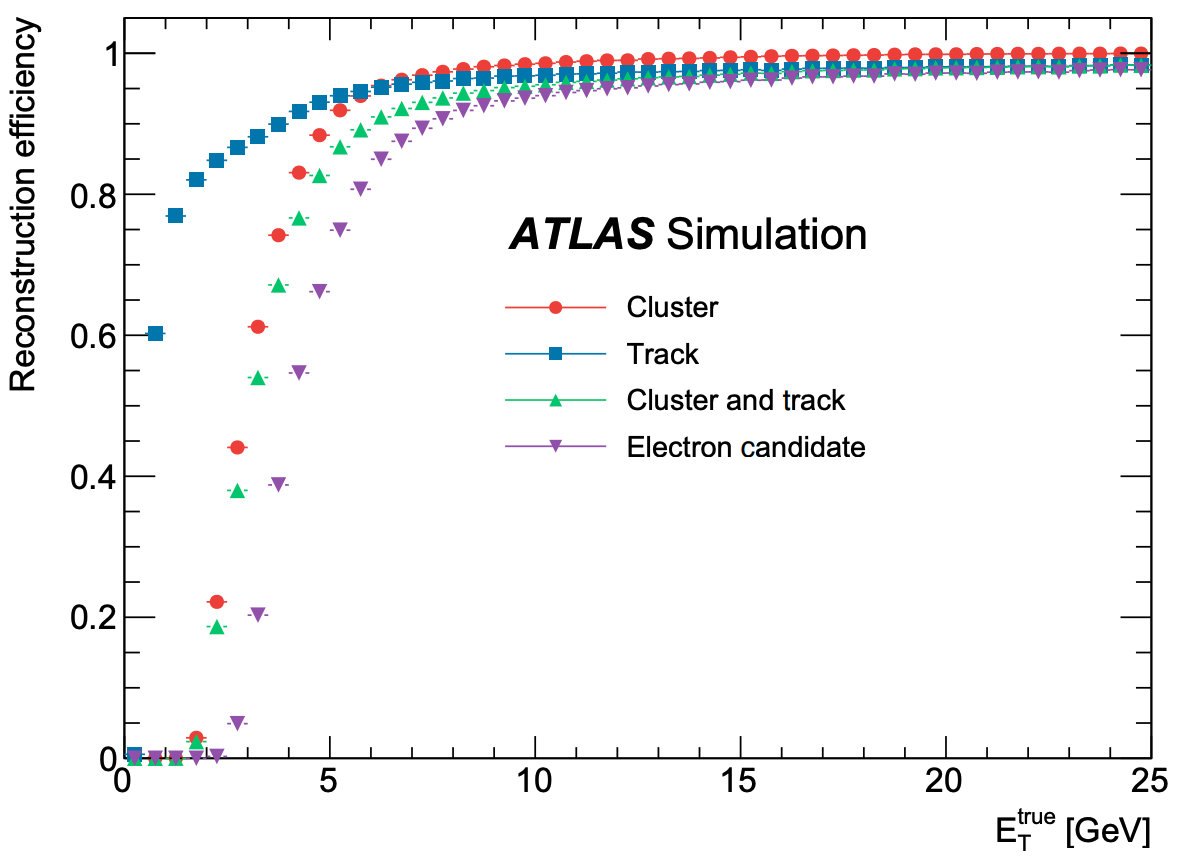
\includegraphics[width=.65\textwidth]{chapters/chapter3_eventreco/images/electron-efficiency.png}

    \caption[The reconstruction efficiency for electrons as a function of true \et.]{The reconstruction efficiency for electrons as a function of true \et for a single-electron sample. Each step of the candidate formation is shown \cite{electron-efficiency}.}
    \label{fig:electron-eff}
\end{figure}


\subsection{Photons} 

Photon reconstruction is very similar to that of electrons. Photons, however, do not interact with the inner tracker material, 

\subsection{Jets}
Strongly interacting particles 

The primary jet identification algorithm in ATLAS is the anti-$k_T$ algorithm REFERENCE and explain. This parameter is set with distance parameter $R=0.4$.

\subsubsection{Jet Flavor Tagging}
\subsection{Muons}
